\subsection{Measurements of the three parallelisation implementations}

We have compared three different parallelisation implementation: 
\begin{enumerate}
\item naive OpenMP which encloses the map step with \texttt{\#pragma omp parallel\#pragma
    omp for} and protects the global result associative array (reduction step) with \texttt{\#pragma omp critical}
\item improved OpenMP, refactored the reduction step by first
  performing a thread-wise reduction in a thread-private associative array and then
  finally reduced in the global result associative array.
\item R automatic multi-threading, an R-side parallelism which uses a \texttt{mclapply} call from the R
\texttt{parallel} package.
\end{enumerate}
\begin{figure}[!htbp] \centering
  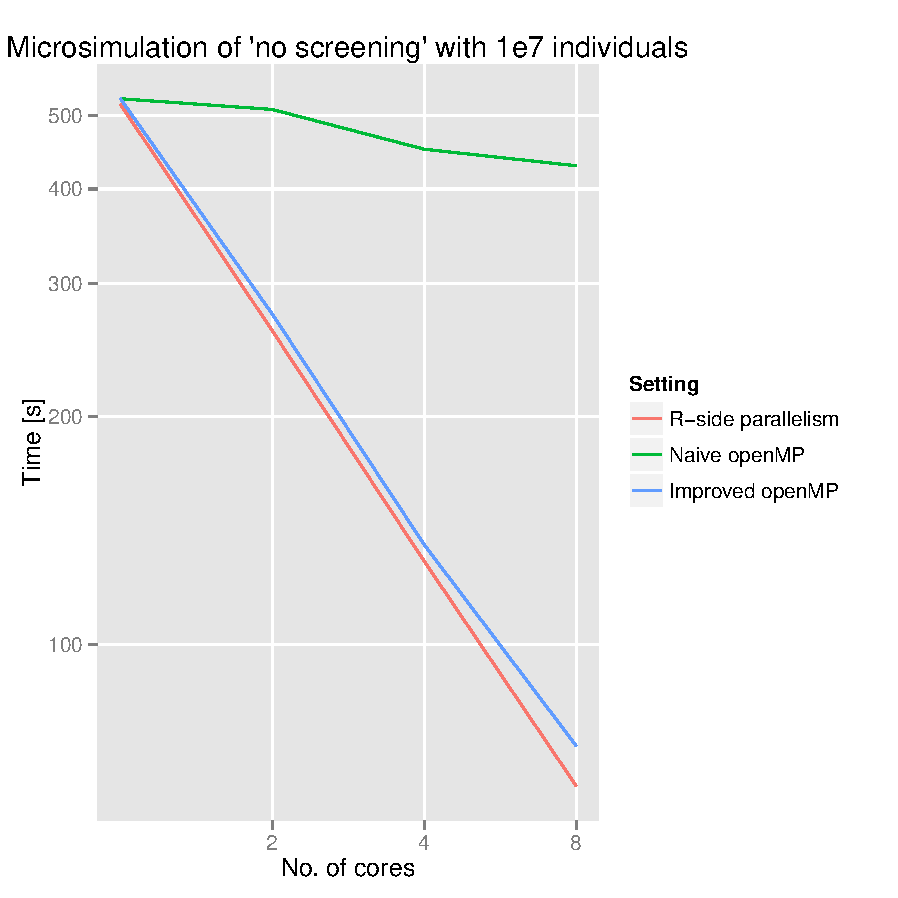
\includegraphics[height=0.5\textheight]{images/implementationProfiling.pdf}
  \caption{implementations...}
  \label{fig:implScaling}
\end{figure} 
Figure \ref{fig:implScaling} shows how the three
different implementations of parallelisation scales with additional
cores. The \emph{R-side parallelism} and \emph{Improved openMP} scales
well with comparable results. The \emph{Naive openMP} implementation
with the \emph{EventReport} mentioned in \ref{fig:cppMot} within
\emph{\#pragma omp critical} statements.



%%% Local Variables: 
%%% mode: latex 
%%% TeX-master: "report" 
%%% End:
